
%%----------------------------------------%%
\begin{frame}
  \frametitle{Dose Contributors, PWR SNF In Yucca}
\footnotesize{
  \begin{figure}[htbp!]
  \begin{center}
    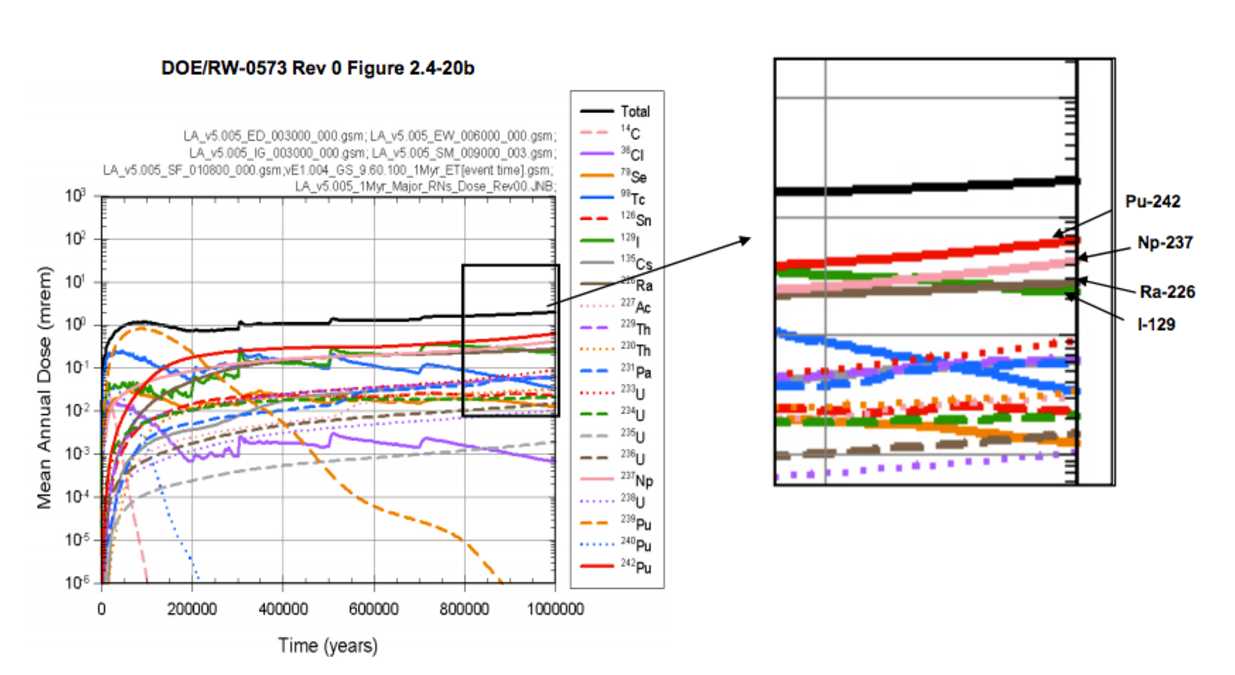
\includegraphics[width=0.7\textwidth]{./images/swift_dose_yucca.eps}
  \end{center}
  \caption{Dose contributors expected in the Yucca Mountain repository 
    \cite{swift_applying_2010}. In the oxidizing environment at Yucca mountain, 
    actinides such as $^{242}Pu$ and $^{237}Np$ dominate dose contribution. We 
    also see that long-lived, highly soluble $^{129}I$ and highly soluble 
    $^{226}Ra$ are also primary dose contributors.}
  \label{fig:swift_dose_yucca}
\end{figure}

}
\end{frame}

%%----------------------------------------%%
\begin{frame}
  \frametitle{Dose Contributors, PWR SNF In Clay}
\footnotesize{
  \begin{figure}[htbp!]
  \begin{center}
    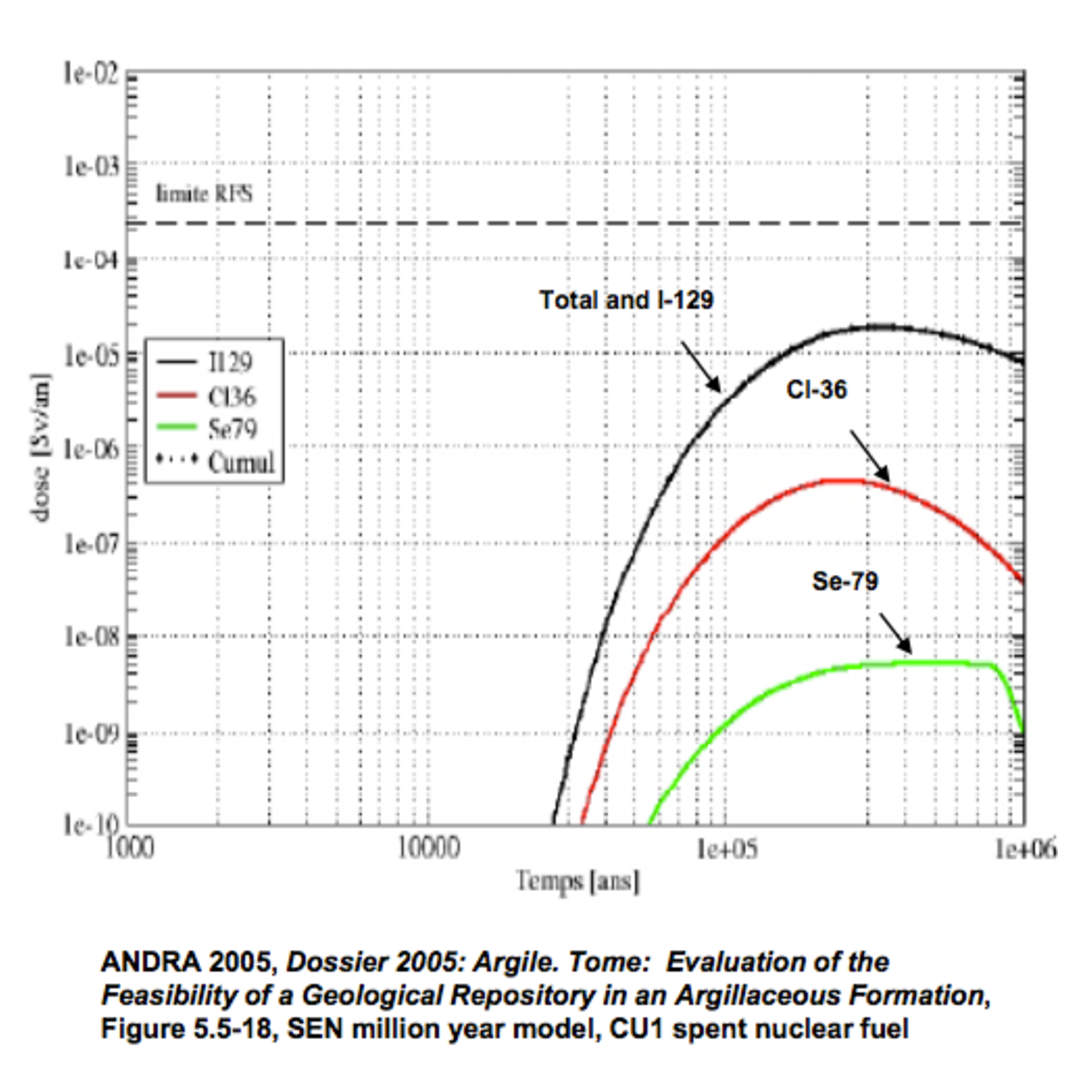
\includegraphics[width=0.5\textwidth]{./images/swift_clay_dose.eps}
  \end{center}
  \caption{Dose contributors expected in a clay repository concept 
    \cite{swift_applying_2010}. Primary contributors are highly soluble, long 
    lived isotopes $^{129}I$, $^{36}Cl$, and $^{79}Se$ .}
  \label{fig:swift_clay_dose}
\end{figure}

}
\end{frame}

%%----------------------------------------%%
\begin{frame}
  \frametitle{Dose Contributors, PWR SNF In Granite}
\footnotesize{
  \begin{figure}[htbp!]
  \begin{center}
    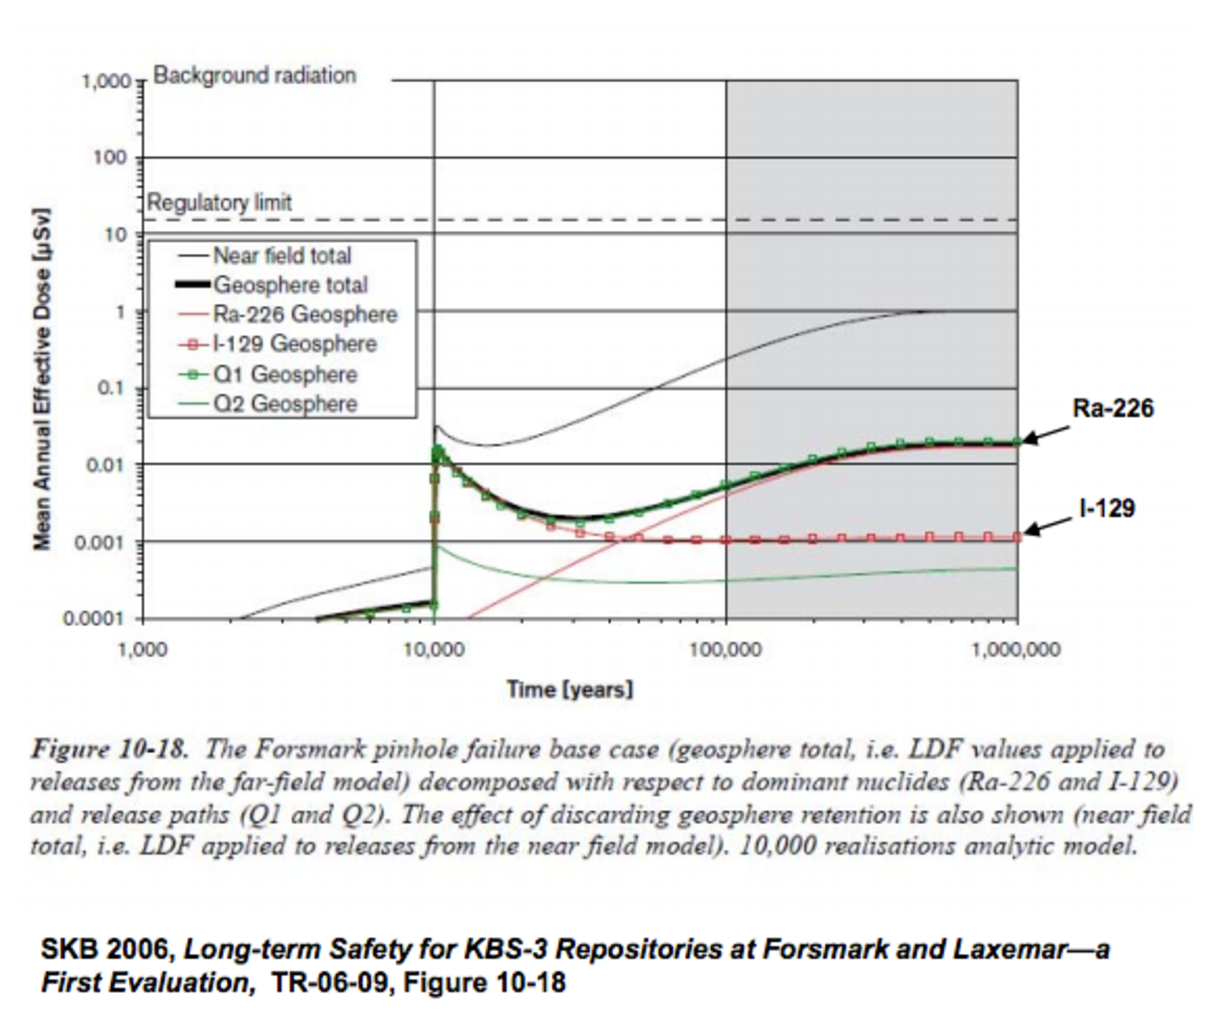
\includegraphics[width=0.7\textwidth]{./images/swift_granite_dose.eps}
  \end{center}
  \caption{Dose contributors expected in a granite repository concept 
    \cite{swift_applying_2010}. Primary contributors in this more advective 
  system are the most mobile products at the time of waste package failure. 
  $^{129}I$ is always a primary contributor.}
  \label{fig:swift_granite_dose}
\end{figure}

}
\end{frame}

%%----------------------------------------%%
\begin{frame}
  \frametitle{Summary: Dose Contributing Isotopes in Various Geologies}
Dominant dose contributors vary among geologies due to both \textbf{water chemistry (sorption, solubility)} and \textbf{transport regime (diffusive, advective)}. 
\begin{itemize}
  \item Long lived, highly soluble, non sorbing $^{129}I$ is a dominant long-term
contributor in all geologies.
  \item In a tuff geology like Yucca Mountain, which is oxidizing with advective transport, actinides dominate in addition to $^{129}I$.
  \item In granite, a typically reducing geology with advective release pathways, mobile $^{226}Ra$ may be important in addition to $^{129}I$.
  \item In primarily diffusive salt and clay geologies, long-lived, highly soluble, non-sorbing fission and activation products ($^{129}I$, $^{36}Cl$, $^{79}Se$)  dominate. 
\end{itemize}
\end{frame}
